\documentclass[tikz,border=8pt]{standalone}
\usepackage{amsmath,amssymb}
\usetikzlibrary{arrows.meta,calc,decorations.pathreplacing,patterns,shapes.geometric,positioning,shadings}

\begin{document}
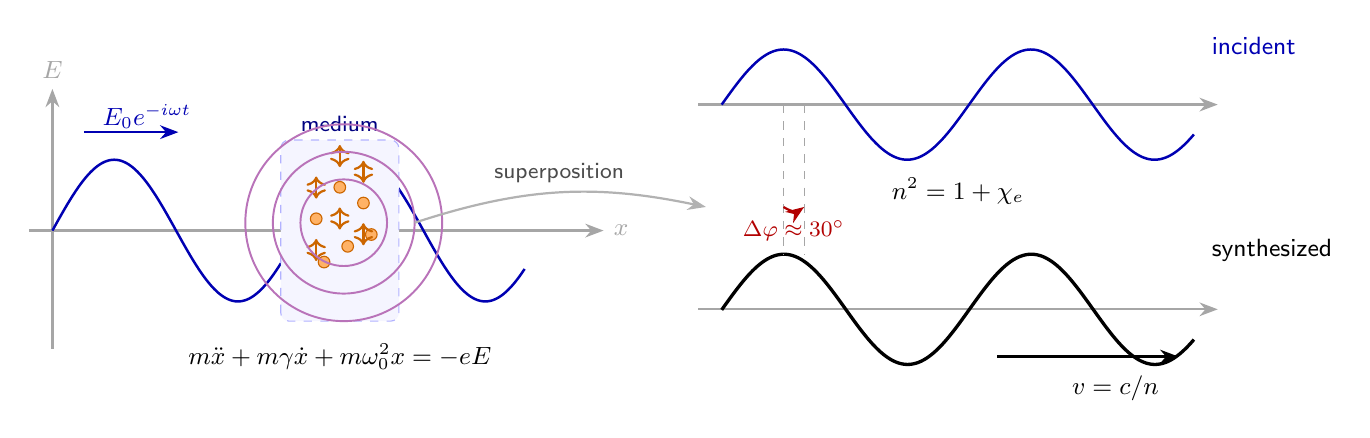
\begin{tikzpicture}[
  font=\sffamily,
  wave/.style={thick, smooth, samples=200, domain=0:6},
  incwave/.style={wave, draw=blue!70!black, line width=0.9pt},
  synthwave/.style={wave, draw=black, line width=1.2pt},
  secondary/.style={draw=violet!55, line width=0.7pt},
  electron/.style={circle, draw=orange!80!black, fill=orange!60, minimum size=4.2pt, inner sep=0pt},
  axisarr/.style={-Stealth, thick, gray!70},
  label/.style={font=\sffamily\small},
  smalllabel/.style={font=\sffamily\footnotesize}
]

% =========================================================
% LEFT PANEL: Incoming wave + electron cloud + secondary waves
% =========================================================

% Coordinate axis for left scene
\draw[axisarr] (-0.3,0) -- (7.0,0) node[right, label] {$x$};
\draw[axisarr] (0,-1.5) -- (0,1.8) node[above, label] {$E$};

% Incoming EM plane wave (blue sinusoid) -- left portion before medium
\draw[incwave] plot (\x, {0.9*sin(2*\x r)});

% Label incident wave
\node[label, blue!70!black] at (1.2, 1.45) {$E_0 e^{-i\omega t}$};
\draw[-Stealth, blue!70!black, thick] (0.4,1.25) -- (1.6,1.25) node[right, smalllabel] {};

% Medium region: shaded rectangle
\begin{scope}
  \fill[blue!4, rounded corners=3pt] (2.9,-1.15) rectangle (4.4,1.15);
  \draw[blue!30, dashed, rounded corners=3pt] (2.9,-1.15) rectangle (4.4,1.15);
\end{scope}
\node[smalllabel, blue!50!black] at (3.65, 1.35) {medium};

% Electron cluster (5 electrons)
\node[electron] (e1) at (3.35, 0.15) {};
\node[electron] (e2) at (3.75,-0.2) {};
\node[electron] (e3) at (3.95, 0.35) {};
\node[electron] (e4) at (3.45,-0.4) {};
\node[electron] (e5) at (3.65, 0.55) {};
\node[electron] (e6) at (4.05,-0.05) {};

% Driven oscillation arrows on electrons (vertical double-arrow)
\foreach \n in {e1,e3,e5} {
  \draw[<->, orange!80!black, thick] ([yshift=-5pt]\n.south) -- ++(0,-0.28);
  \draw[<->, orange!80!black, thick] ([yshift=5pt]\n.north) -- ++(0,0.28);
}

% Secondary spherical waves: three concentric arcs emanating
\foreach \r in {0.55, 0.9, 1.25} {
  \draw[secondary] (3.7,0.1) circle (\r);
}

% Lorentz equation below electron cluster
\node[label, align=center] at (3.65,-1.6)
  {$m\ddot{x} + m\gamma\dot{x} + m\omega_0^2 x = -eE$};

% =========================================================
% RIGHT PANEL: Incident vs Synthesized waves (phase shift)
% =========================================================

% Offset origin for comparison panel
\begin{scope}[xshift=8.5cm]

  % Upper sinusoid: incident (blue)
  \draw[axisarr] (-0.3, 1.6) -- (6.3, 1.6);
  \draw[incwave, domain=0:6]
    plot (\x, {1.6 + 0.7*sin(2*\x r)});
  \node[label, blue!70!black, anchor=west] at (6.1, 2.35) {incident};

  % Lower sinusoid: synthesized (black), phase-shifted by ~30 deg lag
  \draw[axisarr] (-0.3, -1.0) -- (6.3, -1.0);
  \draw[synthwave, domain=0:6]
    plot (\x, {-1.0 + 0.7*sin(2*\x r - 0.5236)});
  \node[label, anchor=west] at (6.1,-0.25) {synthesized};

  % Vertical guide lines showing phase lag at x around pi/4 (peak)
  % Incident peak at 2x = pi/2 -> x = pi/4 ~ 0.785
  % Synth  peak at 2x - pi/6 = pi/2 -> x = pi/3 ~ 1.047
  \draw[dashed, gray!70] (0.785, 1.6) -- (0.785, -1.0+0.7);
  \draw[dashed, gray!70] (1.047, 1.6) -- (1.047, -1.0+0.7);

  % Phase lag arc annotation
  \draw[-Stealth, red!70!black, thick]
    (0.785, 0.3) to[bend right=35] node[midway, below, smalllabel, red!70!black] {$\Delta\varphi \approx 30^{\circ}$} (1.047, 0.3);

  % Label formula n^2 = 1 + chi_e
  \node[label] at (3.0, 0.5) {$n^2 = 1 + \chi_e$};

  % Phase velocity label
  \node[label] at (5.0,-2.0) {$v = c/n$};
  \draw[-Stealth, thick] (3.5,-1.6) -- (5.8,-1.6);

\end{scope}

% Connector arrow from medium region to right panel
\draw[-Stealth, thick, gray!60]
  (4.6, 0.1) to[bend left=15] node[midway, above, smalllabel, gray!60!black] {superposition} (8.3, 0.3);

\end{tikzpicture}
\end{document}
